Le contexte physique naturel des équations d'advection, diffusion, réaction est le suivant:
des particules sont placées dans un milieu fluide où elles \textbf{diffusent}. Ce milieu fluide
est en mouvement, il déplace les particules, les \textbf{advecte}.
Enfin les particules \textbf{réagissent} entre elles et ces réactions modifient les grandeurs thermodynamiques (température, pression) et \textit{in fine} les propriétés
du milieu fluide.
Les équations d'advection, diffusion, réaction modélisent le couplage trois phénomènes.\par 
Cette partie présente les propriétés trois opérateurs des équations d'ADR (\ref{par:adr_3_operator}) et
les difficultés liées à leur résolution numérique (\ref{par:adr_difficile}).

\subsection{Trois opérateurs au propriétés mathématiques très différentes}\label{par:adr_3_operator}
\subsubsection{Advection}
    L'advection désigne le transport d'une quantité par un flot. L'opérateur d'advection le plus simple est l'opérateur
    de transport $c \frac{\partial}{\partial x}$:
    \begin{align}\frac{\partial u}{\partial t} = c \frac{\partial u}{\partial x}\end{align}
    De manière générale l'opérateur d’advection d'une quantité $u$ par un flot $\underline a$ s'écrit $\underline a \cdot \underline{\nabla} u$.
    Par exemple dans les équations de Navier-Stokes, le terme $\underline{v} \cdot \underline{\underline \nabla} \, \underline{v}$ modélise 
    la vitesse $\underline v$ transportée par elle même. Une version simplifiée de ce phénomène est l'équation bien connue de Bürgers.\par 
    Le spectre des opérateurs d'advections sont généralement à valeurs propres imaginaires \cite[Chap.~10]{LeVeque2007}.
    Ainsi ils sont peu raides mais résonnants. Les méthodes explicites sont souvent les plus adaptées pour les traiter \cite[Chap.~10]{LeVeque2007}.

\subsubsection{Diffusion}
    La diffusion désigne l'\textit{éparpillement} de particules au sein d'un milieu fluide
    \footnote{En théorie de l'information cela décrit la tendance de l'entropie augmenter et l'information à se moyenner, se flouter.}.
    Ce phénomène est la limite macroscopique du déplacement microscopique
    des particules dû à l'agitation thermique. L'opérateur de diffusion le plus classique est celui de l'équation de la chaleur:
    \begin{align} \frac{\partial u}{\partial t} = D \Delta u.\end{align}
    Le spectre de cet opérateur est $\mathbb R^-$ \cite[Chap.~9]{LeVeque2007}, il est donc infiniment raide. 
    L'opérateur discret correspondant ne capte qu'une partie de ce spectre.
    En pratique la raideur de l'opérateur discret augmente de manière quadratique avec la finesse de la discrétisation spatiale \cite[Chap.~9]{LeVeque2007}.\par
    Cet opérateur moyennement raide (comparé aux opérateurs de réaction). Ainsi on pourrait penser qu'une méthode implicite est adéquate. Cependant ce n'est généralement pas le cas.
    En effet le coefficient de diffusion n'est souvent pas uniforme ni isotrope. La structure de la matrice de l'opérateur discrétisé évolue donc et
    à chaque itération il faut inverser un nouvel opérateur implicite. Cette tâche est rendue plus ardue encore car l'opérateur de diffusion couple tout l'espace,
    c'est-à-dire qu'il est non local.
    \footnote{Si l'opérateur de diffusion eût été local il aurait pu être inversé en résolvant plusieurs petits systèmes et ce, potentiellement en parallèle.
    Cela serait bien moins coûteux qu'inverser un grand système. 
    À titre d'exemple, inverser une matrice pleine de taille $10^6$ demande environ $10^{18}$ opérations, alors qu'inverser 100 systèmes de taille $10^4$
    n'en demande $100 \times 10^{12} = 10^{14}$ soit dix mille fois moins. Si ces résolutions sont parfaitement parallélisés, alors l'accélération théorique serait d'un million. Malheureusement comme
    l'opérateur de diffusion couple tout l'espace ce n'est pas possible en dimension deux et trois.},
    il faut inverser une matrice de taille $d >> 1$ dont la structure
    peut être très hétérogène (car le coefficient de diffusion varie dans l'espace). Aujourd'hui il semble plus pertinent
    d'utiliser des méthodes explicites stabilisées qui peuvent gérer sa raideur relative comme les méthodes 
    ROK2 et ROK4\cite{abdulle2002fourth}. Sans entrer dans les détails, la clé de ces méthodes consiste à prendre une méthode numérique explicite standard et lui ajouter des étages 
    de sorte à ce que la fonction d'amplification résultante soit la fonction d'amplification de la méthode standard multipliée par un polynôme minimal sur $\mathbb R^-$
    comme un polynôme de Tchebichev.

\subsubsection{Réaction}
    Les phénomènes de réaction sont en général bien adaptés aux méthodes implicites car ils sont locaux et extrêmement raides.
    En effet, les temps typiques d'une réaction chimique\footnote{
    En réalité une réaction chimique aussi simple en apparence qu'une combustion $H_2/O_2$ fait intervenir une dizaine de composés et réactions intermédiaires \cite{OConaire2004}, dont les temps typiques sont très faibles.} sont de l'ordre de la nano-seconde \cite{Wartha2021}.
    %AFAIRE AJOUTER UNE JUSTIFICATION
    De fait, les réactions chimiques sont très difficiles à simuler par des méthodes explicites.
    En revanche les méthodes implicites sont très efficaces dans ce contexte. En effet l'inversion de l'opérateur implicite 
    peut être décomposé en plusieurs résolutions de petits systèmes ce qui est moins coûteux et parallélisable. Cela est permis grâce à la localité des réactions chimiques
    (à chaque pas de temps les particules au sein d'une cellule ne réagissent qu'avec les autres particules de la même cellule).
    En pratique cela signifie qu'il est possible de mettre en oeuvre une petite méthode implicite par cellule plutôt qu'une gargantuesque méthode globale; 
    ce qui revient à inverser un opérateur de petite dimension en chaque cellule et non inverser un énorme système.

\subsection{Difficultés mathématiques intrinsèques}\label{par:adr_difficile}
    La simulations des équations d'advection-réaction-diffusion se heurte à deux difficultés majeures, \textbf{le couplage des trois opérateurs} mentionnés précédemment
    et \textbf{le caractère multi-échelles des solutions}.

    \subsubsection{Première difficulté: le couplage des opérateurs}
        Le développement précédent montre que résoudre chaque phénomène individuellement, n'est pas insurmontable. 
        Toutefois, les résoudre tous en même temps, c'est-à-dire les coupler, est en pratique très difficile.
        En effet, lorsque ces trois opérateurs sont couplés, il en résulte un unique opérateur qui doit être traité par une méthode numérique.
        C'est là que surgissent les difficultés: si la méthode est explicite (éventuellement stabilisée), la raideur de la réaction impose des pas de temps extrêmement restrictifs,
        à l'inverse si la méthode est implicite, la non-localité de la diffusion demande l'inversion d'un système de taille déraisonnable. 
        Cette approche naïve, monolithique, n'est donc pas adaptée. Il faut par conséquent, trouver d'autres stratégies.

    \subsubsection{Seconde difficulté: le caractère multi-échelles des solutions}
        Les solutions étudiées sont souvent multi-échelles, en temps \underline{et} en espace. Cela signifie que certaines zones spatio-temporelles requièrent
        une finesse d'approximation élevée pour pouvoir reproduire fidèlement le comportement physique, tandis qu'en d'autres zones une approximation
        grossière est suffisante. Prenons l'exemple d'un incendie. Au début le foyer est très restreint et seule cette zone doit être maillée finement, 
        car partout ailleurs \textit{il ne se passe rien}. Petit à petit l'incendie se propage et la zone à mailler finement augmente. Un autre exemple de phénomène 
        multi-échelle est la détonation, il faut mailler finement, au foyer de l'explosion et le front de l'onde de choc. Mais la zone non atteinte par l'explosion, 
        qui n'a pas encore reçu le choc, pourrait être maillée très grossièrement. 
        Dans ces conditions, il est imaginable qu'un maillage naïf mène à ce qu'en certains instants, 90\% du domaine soit maillé avec un pas d'espace 100 fois plus fin que nécessaire,
        or en trois dimension mailler 100 fois trop finement multiplie par un million le nombre de cellules.
        Il y a alors une grande inefficacité computationnelle.


% \subsection{Les stratégies de simulation}
%     Pour surmonter ces difficultés, il est d'usage d'utiliser de concert des stratégies d'adaptation de maillage et d'intégration en temps spécifiques. 
%     \subsubsection{L'adaptation de maillage}
%     Pour tirer parti du caractère multi-échelle des solutions, il est courant de recourir à des méthodes d'adaptation de maillage.
%     C'est-à-dire d'employer une résolution variable pour la grille de calcul selon les différentes zones du domaine. 
%     L'adaptation doit se mettre à jour au fil des itérations pour suivre la dynamique de la solution car la répartition de la complexité physique évolue tout au long de la simulation.
%     La méthode d'adaptation de maillage sur laquelle le stage se concentre est la multirésolution-adaptative par transformée d'ondelettes introduite par Ami Harten dans les années 1990 \cite{harten1994}.
%     Cette méthode est très étudiée par l'équipe du CMAP et a donné lieu au développement du logiciel Samurai\footnote{\href{https://github.com/hpc-maths/samurai}{https://github.com/hpc-maths/samurai}}.
%     \begin{figure}[h]
%     \centering
%     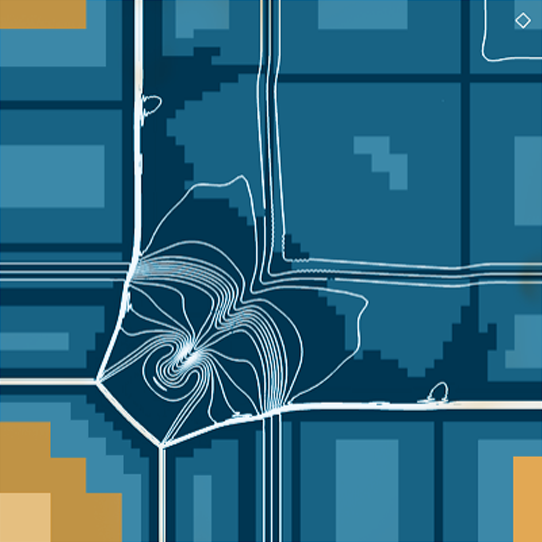
\includegraphics[width=0.5\textwidth]{media/3_/3_/exemple_compression_samurai.png}
%     \caption{Exemple de maillage adapté par multirésolution adaptative grâce au logiciel \href{https://github.com/hpc-maths/samurai}{Samurai}.}
%     \label{fig:samurai}
%     \end{figure}

%         \paragraph{La multi-résolution adaptative}
%         La multirésolution adaptative se base sur une compression de la solution par transformée d'ondelettes\footnote{C'est le même procédé qui est à l'oeuvre dans la compression d'image \texttt{jpg}.}.
%         Les détails mathématiques sont donnés plus tard et s'appuient notamment sur \cite{postePoly} mais pour résumer, la compression se fait de la manière suivante:
%         une transformée multi-échelle sur une base d'ondelettes représente la solution sur différentes échelles d'espace\footnote{Par exemple les échelles $\Delta x, \Delta x/2,\Delta x/4,\dots, \Delta x/2^n$.}. 
%         Cela quantifie l'information portée par chaque niveau de résolution. Enfin la compression consiste à ignorer les échelles comprenant moins d'information
%         qu'un seuil de compression $\varepsilon$ fixé par l'utilisateur.

%         \paragraph{Autres méthodes}
%         Il existe d'autres stratégies pour raffiner la grille de calcul que la multirésolution adaptative.
%         La plus classique est l'adaptation basée sur la magnitude des gradients de la solution. Une grande magnitude des gradients révèle une complexité locale de la solution,
%         appelant une fine résolution du maillage. Cette approche est simple à mettre en oeuvre et part de la même heuristique 
%         que la multirésolution adaptative (détecter où se trouve la complexité de la solution), cependant elle est moins systématique (pas de quantification intrinsèque de l'information perdue) et plus difficile à analyser. 
%         Elle est cependant utilisée dans des logiciels industriels comme Ansys 
%         \footnote{\href{https://w.ww.ansys.com/fr-fr/blog/how-to-accelerate-ansys-fluent-simulations-with-adaptive-meshing}{https://www.ansys.com/fr-fr/blog/how-to-accelerate-ansys-fluent-simulations-with-adaptive-meshing}}.
%         % AFAIRE : ajouter une ref pour les adaptations basées sur les gradients, une justification sur le caractère moins facile a analyser et éventuellement d'autres méthodes de raffinement.

%     \subsubsection{Les techniques d'intégration}
%         Comme expliqué précédemment, la simulation de chaque phénomène intervenant dans les problèmes d'advection-diffusion-réaction est aisée individuellement mais très difficile conjointement.
%         Des stratégies pour intégrer les trois opérateurs en même temps sont donc nécessaires. Elles reposent en réalité sur le fait d'intégrer chaque opérateur... séparément (ou presque).

%         \paragraph{La séparation d'opérateurs}
%             La séparation d'opérateurs (en Anglais: \textit{operator splitting}) consiste à intégrer successivement chaque opérateur.
%             L'intégration d'un opérateur $A$, dans une équation comme :
%             \begin{align}\frac{\partial u}{\partial t} = Au.\end{align}
%             Peut s'écrire formellement avec la notion d'exponentielle de matrice\footnote{Ou de manière plus rigoureuse et plus générale avec la notion de semi-groupe.}:
%             \begin{align}u(\Delta t) = e^{\Delta tA}u_0.\end{align}
%             Si deux opérateurs $A$ et $B$ interviennent dans l'EDP cela donne:
%             \begin{align}\frac{\partial u}{\partial t} = (A+B)u.\end{align}
%             \begin{align}u(\Delta t) = e^{\Delta t (A+B)}u_0 \end{align}
%             Il est alors tentant d'écrire:
%             \begin{align}u(\Delta t)\approx e^{\Delta t(B)}e^{\Delta t(A)}u_0.\end{align}
%             Ce n'est malheureusement qu'une approximation car $e^{\Delta t(A+B)} = e^{\Delta t(B)}e^{\Delta t(A)}$ n'est vrai que si les opérateurs $A$ et $B$ commutent.
%             Cependant c'est vrai à l'ordre $O(\Delta t)$. 
%             Il est donc possible de simuler le problème en séparant les opérateurs de la manière suivante: 
%             \begin{align}
%                 \text{Étape 1: simuler }&v=e^{\Delta t A}u^n,\notag\\\notag
%                 \text{Étape 2: simuler }&u^{n+1}=e^{\Delta t B}v,\\
%             \end{align}
%             Cet algorithme correspond au schéma de splitting de Lie, introduisant une erreur de l'ordre $\Delta t$. 
%             Il existe un autre schéma: le splitting de Strang qui est précis à l'ordre $\Delta t^2$ grâce au développement $e^{\Delta t (A+B)} = e^{\Delta t B}e^{\Delta t A} e^{\Delta t B}$.
%             Ces méthodes de séparation d'opérateurs, très simples à mettre en oeuvre, permettent de traiter les opérateurs indépendamment les uns à la suite des autres; chacun avec une méthode numérique adaptée.
%             Malheureusement elles sont aveugles à certains couplages entre les différents phénomènes modélisés et il est difficile de monter au-delà de l'ordre deux en temps. La promesse des
%             approches ImEx présentées par la suite est de combler ces lacunes.\par
%             % AFAIRE --> quels sont les éventuels phénomènes de couplages ? En quoi c'est un problème si l'ordre est formellement bon ?
%             Une étude extensive de l'usage du splitting, pour les équations d'advection-diffusion-réaction couplées à la multirésolution adaptative 
%             a été réalisée dans la thèse de Max Duarte, préparée à Centrale Paris sous la direction de Marc Massot \cite{duart2011}.
%             Cela a montré que les techniques d'opérateurs sont très efficaces mais qu'en pratique, une perte de l'ordre formel peut avoir lieu.

%         \paragraph{Les méthodes ImEx}
%             Ces méthodes sont détaillées en \ref{par:ImEx_presentation}. Ces méthodes ImEx
%             \footnote{Les méthodes présentées ici sont les méthodes ImEx Runge et Kutta (RK-ImEx). Il existe également des approches ImEx couplées espace-temps\cite{rebou2024}.}  \cite{pareschi2010implicitexplicitrungekuttaschemesapplications} \cite{KENNEDY2003139}
%             sont très proches de la séparation d'opérateurs lors de l'implémentation. Toutefois, elles apportent plus de cohérence mathématique
%             et facilitent la montée en ordre. 
%             Une méthode Runge et Kutta est une technique d'intégration en temps dont chaque itération se décompose en plusieurs étapes (aussi appelées étages).
%             Chaque étage engendre une nouvelle approximation, puis en fin d'itération une combinaison linéaire des ces approximations intermédiaires donne la solution au pas de temps suivant.
%             Cette approche permet de monter en ordre efficacement.
%             Dans les méthodes Runge et Kutta ImEx à chaque étage, l'approximation associée est obtenue en ajoutant d'une part des contributions explicites des opérateurs pour lesquels les méthodes explicites sont adaptées,
%             et d'autre part des contributions implicites des opérateurs pour lesquels les méthodes implicites sont adaptées.
%             Ainsi, un traitement différent est appliqué à chaque opérateur tout en conservant une approche globalement cohérente\footnote{Cependant les méthodes de splitting 
%             offrent le luxe de choisir chaque technique de résolution numérique indépendamment des autres, ici ce n'est plus le cas des relations d'ordre doivent être respectées;
%             plus de cohérence mais plus de contrainte.}.
%             % AFAIRE AJOUTER UN LIEN VERS LE CHAPITRE DÉDIÉ
%             % AFAIRE SE DEMANDER SI POUR U? OPÉRATEUR LINÉAIRE RKImEx ET SPLITTING C EST PAREIL MAIS SI LE RKImEx NE SERAIT PAS PLUS PERTINENT EN NON LINÉAIRE.

\subsection{Conclusion sur les équations d'ADR}
Les solutions multi-échelles ainsi que le couplage des trois opérateurs
rendent les équations d'advection-diffusion-réaction difficiles à résoudre numériquement.
D'une part les trois ne peuvent être traitées efficacement par une approche monolithique classique. 
D'autre part, le caractère multi-échelle tend au gaspillage de ressources de calculs.
Cette dernière difficulté pousse les numériciens vers des stratégies d'adaptation en espace, 
celle étudiée dans ce stage est la multi-résolution adaptative (MRA) dont les détails techniques sont donnés à la section suivante.